\documentclass[notes]{beamer}
%\documentclass[11pt,letterpaper]{article}
%\usepackage{beamerarticle}

\usepackage{genchem-lecture}
\usepackage{ccicons}

\title{The Quantum-Mechanical Model of the Atom}
\subtitle{Chapter 2}
\institute[CHEM115 Bloomsburg University]{CHEM115 --- Chemistry for the Sciences I \\ Bloomsburg University}
\author{CHEM115 - Chemistry for the Sciences I}
\date{Spring 2019}

\begin{document}

\begin{frame}
	\titlepage
\end{frame}

\begin{frame}{Schrodinger's Cat}
	\centering
	\includegraphics[scale=0.2]{Schrodingers-cat.pdf}

	\footnotesize \ccbysa\ Dhatfield
\end{frame}

\begin{frame}{The Nature of Light}
	\begin{block}{Particle-Wave Duality}
		Light (and electrons as we'll see later) is both a particle and
		a wave.
	\end{block}

	\begin{center}
		\includegraphics[scale=0.4,trim={0 0 0 40pt},clip]{emrad.jpeg}
	\end{center}

	\begin{itemize}
		\item All electromagnetic waves move through space (in a vacuum)
			at the same, constant speed of
			\emph{\SI{3.00e8}{\meter\per\second}}.
	\end{itemize}
\end{frame}

\begin{frame}[allowframebreaks]{Properties of Waves}
	\begin{center}
		\includegraphics[scale=0.4]{wave-props.jpeg}
	\end{center}

	\begin{description}
		\item[Wavelength ($\lambda$):] the distance between two peaks
			(maxima).
		\item[Amplitude:] vertical height of the peak.
		\item[Frequency ($\nu$):] the number of cycles (peaks) to pass
			through a stationary point in a given time period.
	\end{description}

	\framebreak

	\begin{center}
		\includegraphics[scale=0.4]{wave-props2.jpeg}
	\end{center}
\end{frame}

\begin{frame}{Finding Relationships via Dimensional Analysis}
	\only<presentation:1|article:0|handout:0>{
		\begin{center}
			\includegraphics[scale=0.4]{relationship.pdf}
		\end{center}}

	\pause

	We have\ldots

	\begin{center}
		\tabulinesep=0.5em
		\begin{tabu} spread 30pt {>{\ldots~}X[-1]  X[-1,c] X[-1,c] X[l]}
			wavelength     & $\lambda$ & \si{\nano\meter      } & length \\
			frequency      & $\nu    $ & \si{1\per\second     } & time \\
			speed of light & $c      $ & \si{\meter\per\second} & length and time \\
		\end{tabu}
	\end{center}

	\pause

	\begin{equation*}
		c = \lambda v \qquad\text{\em or}\qquad \lambda = \frac{c}{\nu} \qquad\text{\em or}\qquad \nu = \frac{c}{\lambda}
	\end{equation*}
\end{frame}

\begin{frame}{The Electromagnetic Spectrum}
	Different $\lambda$ of light correspond to different energy regions of
	the electromagnetic spectrum.
	\begin{center}
		\includegraphics[scale=0.45,trim={0 0 0
		30pt},clip]{emspectrum.jpeg}
	\end{center}
\end{frame}

\begin{frame}
	Consider these two waves:

	\bigskip

	\begin{columns}
		\column{0.5\linewidth}
	\begin{center}
		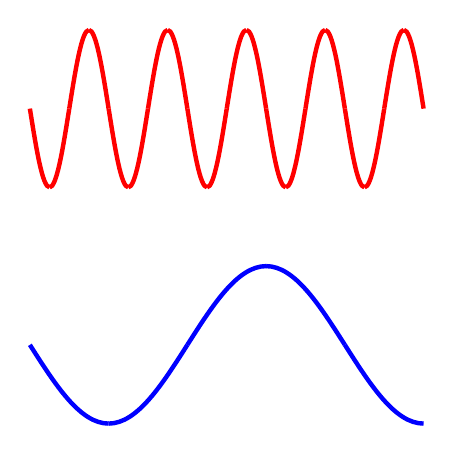
\begin{tikzpicture}
			\foreach \x in {0,1,...,4}{
				\draw[ultra thick, red] (\x,0) sin (\x+0.25,-1);
				\draw[ultra thick, red] (\x+0.25,-1) cos (\x+0.5,0);
				\draw[ultra thick, red] (\x+0.5,0) sin (\x+0.75,1);
				\draw[ultra thick, red] (\x+0.75,1) cos (\x+1,0);
				};
			\draw[ultra thick, blue] (0,-3) sin (1,-4);
			\draw[ultra thick, blue] (1,-4) cos (2,-3);
			\draw[ultra thick, blue] (2,-3) sin (3,-2);
			\draw[ultra thick, blue] (3,-2) cos (4,-3);
			\draw[ultra thick, blue] (4,-3) sin (5,-4);
		\end{tikzpicture}
	\end{center}
		\column{0.4\linewidth}

	\begin{enumerate}[<+(1)->]
		\item Which has the higher frequency?
		\item If one of these represents visible light and the other IR
			radiation, which is which?
	\end{enumerate}
	\end{columns}
\end{frame}

\begin{frame}[t]
	A photon has a frequency of \SI{6.0e14}{\hertz}. Convert this frequency
	into wavelength (\si{\nano\meter}). Does this frequency fall in the
	visible region? ($c = \SI{3.0e8}{\meter\per\second}$)

	\note{
		\begin{tabu} to \linewidth {@{}*{3}{X[c]}}\savetabu{giveplanfind}
			\toprule\rowfont{\bfseries} Given & Plan & Find \\ \midrule
			\SI{6.0e14}{\hertz}      & $c = \SI{3.00e8}{\meter\per\second}$ & \si{\nano\meter} \\
			\SI{6.0e14}{\per\second} & $\SI{1e9}{\nano\meter} = \SI{1}{\meter}$ \\
			\bottomrule
		\end{tabu}

		\begin{align*}
			\frac{\num{6.0e14}}{\si{\second}} \times \frac{\si{\second}}{\SI{3.00e8}{\meter}} \times \frac{\SI{1}{\meter}}{\SI{1e9}{\nano\meter}} &= \SI{0.002}{\per\nano\meter} \\
			(\SI{0.002}{\per\nano\meter})^{-1} &= \SI{500}{\nano\meter} \\
			&= \boxed{\SI{5.0e2}{\nano\meter}}
		\end{align*}

		\fbox{Yes.}
		}
\end{frame}

\begin{frame}{The Wave Nature of Light}{Interference}
	\centering

	\includegraphics[scale=0.4]{constructive-interference.jpeg}

	\bigskip

	\includegraphics[scale=0.4]{destructive-interference.jpeg}
\end{frame}

\begin{frame}{The Wave Nature of Light}{Diffraction}
	\centering
	\only<1>{\includegraphics[scale=0.4]{diffraction.jpeg}}

	\only<2>{\includegraphics[scale=0.4]{diffraction-interference.jpeg}}
\end{frame}

\begin{frame}{The Particle Nature of Light}{The Photoelectric Effect}
	\begin{center}
		\includegraphics[scale=0.4,trim={0 20pt 0 40pt},clip]{photoelectric-effect.jpeg}
	\end{center}

	\begin{description}
			\only<1>{
		\item[Theory:] Energy from light would need to exceed binding
			energy of electron.
			\begin{itemize}
				\item Short $\lambda$, high energy light
				\item Long $\lambda$, low energy light over
					extended time
			\end{itemize}}
			\only<2>{
		\item<2>[Observation:] No matter how long the low energy light was
			used, electrons were not emitted.}
	\end{description}
\end{frame}

\begin{frame}{The Quantum Nature of Light}{Einstein's Explanation}
	\begin{itemize}
		\item Light is composed of photons -- ``packets'' of a specific
			energy (\emph{quantized})
		\item Depend only on frequency, $E = h \nu$
			\begin{itemize}
				\item inversely proportional to $\lambda$
				\item proportionality constant -- \emph{Planck's
					Constant ($h$)}

					\begin{equation*}
						h =
						\SI{6.626e-34}{\joule\second}
					\end{equation*}
			\end{itemize}
	\end{itemize}
\end{frame}

\begin{frame}{A little rearrangement\ldots}
	\begin{align*}
		\intertext{From before:}
		\nu &= \frac{c}{\lambda} \\
		\visible<2->{\intertext{We now have:}
		E &= h\nu \\}
		\visible<3->{\intertext{Therefore,}
		E &= \frac{hc}{\lambda}}
	\end{align*}
\end{frame}

\stepcounter{theexample}
\begin{frame}[t]{\numexample}
	\parbox[t][14em]{\linewidth}{
	When copper is bombarded with high-energy electrons, X-rays are emitted.
	Calculate the energy (in \si{\joule}) associated with the photons if the
	wavelength of the X-rays is \SI{0.154}{\nano\meter}. ($h =
	\SI{6.63e-34}{\joule\second}$)}

	\note{
		\begin{tabu}{\usetabu{giveplanfind}}
			\toprule\rowfont{\bfseries} Given & Plan & Find \\ \midrule
			$\lambda = \SI{0.154}{\nano\meter}$ & $E = \frac{hc}{\lambda}$ & \si{\joule} \\
			\bottomrule
		\end{tabu}

		\begin{align*}
			E &= \frac{hc}{\lambda} \\
			&= \frac{(\SI{6.63e-34}{\joule\second})(\SI{3.00e8}{\meter\per\second})}{\SI{0.154}{\nano\meter}} \times \frac{\SI{1e9}{\nano\meter}}{\SI{1}{\meter}} \\ &= \SI{1.29156e-15}{\joule} \\
			&= \boxed{\SI{1.29e-15}{\joule}}
		\end{align*}
			}
\end{frame}

\stepcounter{theexample}
\begin{frame}[t]{\numexample}
	\parbox[t][14em]{\linewidth}{Calculate the energy of a photon with a frequency of
	\SI{5.09e13}{\per\second}. How much energy would \SI{1}{\mole} of these
	photons contain?}

	\note{
		\begin{tabu} to \linewidth {@{}X[-1,c] X[-1,c] X[-1,c]}
			\toprule\rowfont{\bfseries} Given & Plan & Find \\ \midrule
			$\nu = \SI{5.09e13}{\per\second}$ & $E = h \nu$  & \si{\joule\per\mole} \\
			& $\SI{1}{\mole} = \num{6.022e23}$ \\
			& $h = \SI{6.63e-34}{\joule\second}$ \\
			\bottomrule
		\end{tabu}

		\begin{align*}
			E_{\SI{1}{photon}} &= h\nu
			= (\SI{6.63e-34}{\joule\second})(\SI{5.09e13}{\per\second}) \\
			&= \SI{3.37467e-20}{\joule} \\
			E_{\SI{1}{\mole}} &= \SI{3.37467e-20}{\joule\per photon} \times \frac{\SI{6.022e23}{photons}}{\SI{1}{\mole}} \\
			&= \SI{20315.5134}{\joule\per\mole}
			= \boxed{\SI{20.3e3}{\joule\per\mole}} \\
			\intertext{Often expressed as\ldots}
			&= \boxed{\SI{20.3}{\kilo\joule\per\mole}}
		\end{align*}}


\end{frame}

\begin{frame}[allowframebreaks]{Emission Spectra}
	\centering
	\includegraphics[scale=0.3,trim={0 30pt 0 0},clip]{lamp-emission.jpeg}

	\includegraphics[scale=0.3,trim={0 30pt 0 0},clip]{emission-spectra.jpeg}

	\framebreak

	\includegraphics[scale=0.4]{emission-spectra2.jpg}
\end{frame}

\begin{frame}{Bohr's Model of the Atom (1913)}
	\begin{itemize}
		\item Electrons could only have \emph{very specific amounts} of
			energy.
		\item Electrons traveled in orbits that were a fixed distance
			from the nucleus.
			\begin{itemize}
				\item \emph{Stationary states}
				\item The energy of the electron was
					proportional to the distance the orbital
					was from the nucleus.
			\end{itemize}
		\item Electrons emitted radiation when they ``jumped'' from an
			orbit with higher energy down to an orbit with lower
			energy.
			\begin{itemize}
				\item The distance between the orbits determined
					the energy of the photon of light
					produced.
			\end{itemize}
	\end{itemize}
\end{frame}

\only<presentation|handout:0|article:0>{
\begin{frame}{Orbits?}
	\centering

	\includegraphics[scale=0.8]{stylized-li-atom.pdf}

	\bigskip

	\tiny\ccbysa\ Indolences
\end{frame}}

\begin{frame}
	\centering

	\includegraphics[scale=0.4]{bohr-model.jpeg}
\end{frame}

\begin{frame}{Electron Transitions}
	\begin{columns}
		\column{0.45\linewidth}
		\begin{itemize}
			\item<1-> Electrons can exist \emph{only} in certain
				orbitals (not in between).
			\item<2-> Light \emph{emission} is a result of an
				\emph{electron transition} from a higher energy
				orbital to one of lower energy.
			\item<3-> Ligh \emph{absorption} is a result of an
				\emph{electron transition} from a lower energy
				orbital to one of higher energy.
		\end{itemize}
		\column{0.45\linewidth}
		\begin{center}
		\begin{tikzpicture}[hv/.style={->,decorate,decoration={snake,
			amplitude=2pt,segment length=10pt,post=lineto,post
			length=2pt},red}]
			\draw[very thick,->] (0,-5) -- (0,0) node[midway,left] {$E$};
			\draw[thick] (0.2,-1) -- (1.2,-1) node[at end,right]
			{\emph{Excited State}};
			\draw[thick] (0.2,-4) -- (1.2,-4) node[at end,right]
			{\emph{Ground State}};
			\only<1>{\draw[thick,<->,inner sep=10pt] (0.7,-1.1) --
			(0.7,-3.9) node[midway,right] {$\Delta E$};}
			\only<2|handout:0|article:0>{\draw[thick,->] (0.7,-1.1) -- (0.7,-3.9);
			\draw[hv] (0.8,-2.5) -- (2.3,-2.5) node[midway,above]
			{$h\nu$} node[at end,right] {$\Delta E < 0$};}
			\only<3|handout:0|article:0>{\draw[thick,<-] (0.7,-1.1) -- (0.7,-3.9);
			\draw[hv] (2.3,-2.5) -- (0.8,-2.5) node[midway,above]
			{$h\nu$} node[at start,right] {$\Delta E > 0$};}
		\end{tikzpicture}
		\end{center}
	\end{columns}
\end{frame}

\begin{frame}{Hydrogen Energy Transitions and Radiation}
	\centering
	\includegraphics[scale=0.5,trim={0 0 0 30pt},clip]{H-transitions.jpeg}
\end{frame}

\stepcounter{theexample}
\begin{frame}{\numexample}
	Consider the following energy levels of a hypothetical atom:

	\begin{columns}
		\column{0.45\linewidth}
		\begin{center}
			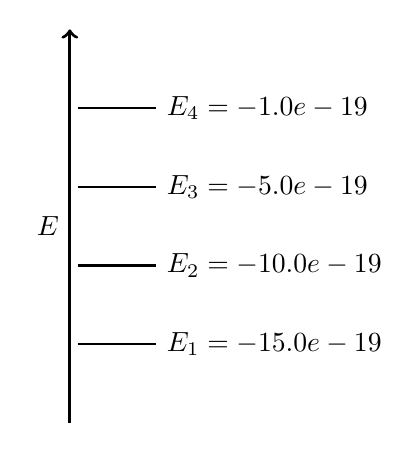
\begin{tikzpicture}
				\draw[very thick,->] (0,-1) -- (0,4) node[midway,left] {$E$};
				\draw[thick] (0.1,3) -- ++(1,0) node[at end,right]{$E_4 = \SI{-1.0e-19}{\joule} $};
				\draw[thick] (0.1,2) -- ++(1,0) node[at end,right]{$E_3 = \SI{-5.0e-19}{\joule} $};
				\draw[thick] (0.1,1) -- ++(1,0) node[at end,right]{$E_2 = \SI{-10.0e-19}{\joule}$};
				\draw[thick] (0.1,0) -- ++(1,0) node[at end,right]{$E_1 = \SI{-15.0e-19}{\joule}$};
			\end{tikzpicture}
		\end{center}
		\column{0.45\linewidth}
		\begin{enumerate}
			\item What is the energy (in \si{\joule}) a photon must
				have in order to excite an electron from $E_2$
				to $E_3$?
				\note[item]{
					\begin{tabu} spread 10pt {c
						S[table-format=2.1e-2]<{
							\si{\joule}}}
							& -5.0e-19 \\
							- &-10.0e-19 \\
							\tabucline-
							& 5.0e-19
					\end{tabu}}
			\item What is the wavelength of the photon emitted when
				an electron goes from $E_4$ to $E_1$?
				\note[item]{
					\begin{tabu} spread 10pt {c
						S[table-format=2.1e-2]<{
							\si{\joule}}}
							& -15.0e-19 \\
							- &-1.0e-19 \\
							\tabucline-
							& 14.0e-19
					\end{tabu}}
		\end{enumerate}
	\end{columns}
\end{frame}

\begin{frame}{Wave Behavior of Electrons}
	\begin{columns}
		\column{0.45\linewidth}
		\begin{itemize} 
			\item Louis de Broglie (1924) -- Particles of \emph{all} sizes
				have both particle and wave properties.
			\item The wave character is only significant for sub-atomic
				particles (very small mass).
			\item Electron beams show an interference pattern!
				\begin{itemize}
					\item The electrons interfere with
						themselves.
				\end{itemize}
			\item<2-> How do we calculate the frequency or
				wavelength of an electron?
		\end{itemize}
		\column{0.45\linewidth}
		\centering
		\includegraphics[scale=0.3]{electron-interference.jpeg}
	\end{columns}
\end{frame}

\begin{frame}{The de Broglie Wavelength}
	de Broglie predicted that the wavelength of a particle was
	\emph{inversely proportional} to its \emph{momentum}:

	\begin{align*}
		\text{Momentum} &= mv \\
		\intertext{where $m$ is mass and $v$ is velocity.}
		\lambda &= \frac{h}{mv} \\
	\end{align*}

	\begin{center}
		\emph{If we know the velocity of an electron, we also know its
		wavelength.}
	\end{center}
\end{frame}

\stepcounter{theexample}
\begin{frame}[t]{\numexample}
	What is the de Broglie wavelength (in \si{\nano\meter}) associated with
	a \SI{143}{\gram} baseball traveling at \SI{40.0}{\meter\per\second}?

	\note{
		\begin{tabu}{\usetabu{giveplanfind}}
			\toprule\rowfont{\bfseries} Given & Plan & Find \\
			\midrule
			$m = \SI{143}{\gram}$ & $\lambda = \frac{h}{mv}$ &
			\si{\nano\meter} \\
			$v = \SI{40.0}{\meter\per\second}$ & $h =
			\SI{6.626e-34}{\joule\second} \\ \bottomrule
		\end{tabu}

		\begin{align*}
			\lambda &=
			\frac{\SI{6.626e-34}{\joule\second}}{(\SI{143}{\gram})(\SI{40.0}{\meter\per\second})}
			\\
			\intertext{Seconds cancels out\ldots but what about
			joules?}
			&= \frac{{\SI{6.626e-34}{\joule\second}}{(\SI{143}{\gram})(\SI{40.0}{\meter\per\second})}
			\times
			\frac{\SI{1}{\kilo\gram\meter\squared\per\second\squared}}{\SI{1}{\joule}}
			\times \frac{\SI{1000}{\gram}}{\SI{1}{\kilo\gram}}
			\times \frac{\SI{1e-9}{\nano\meter}}{\SI{1}{\meter}} \\
			&= \SI{1.15839e-43}{\nano\meter} =
			\boxed{\SI{1.16e-43}{\nano\meter}}
		\end{align*}

		Way to small to ever measure.
\end{frame}

\end{document}
